\documentclass[tikz,border=10pt]{standalone}
\usepackage{amsmath}
\usetikzlibrary{positioning, arrows.meta, shapes, calc}

\definecolor{gnncolor}{RGB}{70,130,180}   % SteelBlue
\definecolor{transcolor}{RGB}{50,205,50}   % LimeGreen
\definecolor{fusioncolor}{RGB}{220,20,60}  % Crimson
\definecolor{structcolor}{RGB}{139,69,19}  % SaddleBrown
\definecolor{seqcolor}{RGB}{255,140,0}     % DarkOrange

\begin{document}

\begin{tikzpicture}[
    node distance=1.2cm and 1.5cm,
    >=Stealth,
    block/.style={rectangle, draw, thick, rounded corners, minimum height=1.2cm, minimum width=2cm, align=center},
    smallblock/.style={rectangle, draw, thick, rounded corners, minimum height=0.8cm, minimum width=1.5cm, align=center},
    graphnode/.style={circle, draw=structcolor, fill=structcolor!20, inner sep=1.5pt},
    seqtoken/.style={rectangle, draw=seqcolor, fill=seqcolor!20, minimum width=8pt, minimum height=16pt},
    fusion/.style={diamond, draw=fusioncolor, fill=fusioncolor!20, thick, inner sep=2pt},
    label/.style={font=\small}
]

% ========================
% INPUTS
% ========================
% Protein structure (schematic)
\node (pdb) [label=below:{PDB Structure}] {
    \begin{tikzpicture}[scale=0.4, every node/.style={scale=0.8}]
        \draw[structcolor, thick] plot[smooth, tension=1] coordinates {(0,0) (0.5,0.8) (1.2,0.6) (1.8,1.2) (2.5,0.9) (3.0,1.5)};
        \foreach \x/\y in {0.5/0.8, 1.8/1.2, 3.0/1.5} {
            \fill[structcolor] (\x,\y) circle (2pt);
        }
    \end{tikzpicture}
};

% Graph from structure
\node[right=1.8cm of pdb] (graph) {
    \begin{tikzpicture}[scale=0.5]
        \node[graphnode] (v1) at (0,0) {};
        \node[graphnode] (v2) at (1,0.8) {};
        \node[graphnode] (v3) at (2,0.3) {};
        \node[graphnode] (v4) at (1.5,-0.5) {};
        \draw[structcolor, thick] (v1) -- (v2) -- (v3) -- (v4) -- (v1);
        \draw[structcolor, thick] (v2) -- (v4);
    \end{tikzpicture}
};
\node[below=0.1cm of graph, font=\small] {Geometric Graph $\mathcal{G}$};

% Sequence
\node[below=2cm of pdb] (seq) {
    \begin{tikzpicture}[scale=0.6]
        \foreach \i/\a in {1/M, 2/T, 3/H, 4/E, 5/L, 6/D, 7/G, 8/A, 9/M, 10/U, 11/T} {
            \node[seqtoken] (s\i) at (\i*0.3,0) {\tiny \a};
        }
        % Highlight mutation
        \node[seqtoken, fill=red!30, draw=red] at (6*0.3,0) {\tiny \textbf{D}};
    \end{tikzpicture}
};
\node[below=0.1cm of seq, font=\small] {Sequence $S$ (mutation at pos 6)};

% ========================
% ENCODERS
% ========================
\node[block, gnncolor, right=1.5cm of graph] (gnn) {Geometric GNN \\ (4 layers)};
\node[block, transcolor, right=1.5cm of seq] (trans) {Transformer \\ (6 layers)};

% Arrows to encoders
\draw[->, thick] (graph) -- (gnn);
\draw[->, thick] (seq) -- (trans);

% ========================
% REPRESENTATIONS
% ========================
\node[smallblock, gnncolor, above=0.8cm of gnn] (z_struct) {$\mathbf{z}_{\text{struct}}$};
\node[smallblock, transcolor, below=0.8cm of trans] (z_seq) {$\mathbf{z}_{\text{seq}}$};

\draw[->, thick, gnncolor] (gnn) -- (z_struct);
\draw[->, thick, transcolor] (trans) -- (z_seq);

% ========================
% DIFFUSIVELY GATED ATTENTION
% ========================
% Structural prior matrix (schematic)
\node[above right=0.5cm and 1cm of z_struct] (Astruct) {
    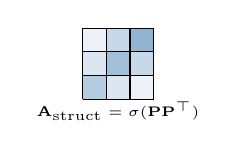
\begin{tikzpicture}[scale=0.3]
        \fill[gnncolor!40] (0,0) rectangle (1,1);
        \fill[gnncolor!20] (1,0) rectangle (2,1);
        \fill[gnncolor!10] (2,0) rectangle (3,1);
        \fill[gnncolor!20] (0,1) rectangle (1,2);
        \fill[gnncolor!50] (1,1) rectangle (2,2);
        \fill[gnncolor!30] (2,1) rectangle (3,2);
        \fill[gnncolor!10] (0,2) rectangle (1,3);
        \fill[gnncolor!30] (1,2) rectangle (2,3);
        \fill[gnncolor!60] (2,2) rectangle (3,3);
        \draw[step=1, black, thin] (0,0) grid (3,3);
        \node at (1.5,-0.5) {\tiny $\mathbf{A}_{\text{struct}} = \sigma(\mathbf{P}\mathbf{P}^\top)$};
    \end{tikzpicture}
};

% Diffusion into attention
\node[fusion, right=1.2cm of z_seq] (dga) {Diffusively \\ Gated \\ Attention};

\draw[->, thick, gnncolor] (z_struct) -| (dga);
\draw[->, thick, transcolor] (z_seq) -- (dga);

% Label for diffusion
\node[above=0.1cm of $(z_struct)!0.5!(Astruct.west)$, font=\scriptsize, gnncolor] {Structural \\ Prior};

% ========================
% FUSION & OUTPUT
% ========================
\node[block, fusioncolor, right=1.5cm of dga] (fusion) {Cross-Modal \\ Fusion};
\node[block, fusioncolor, right=1.5cm of fusion] (pred) {Prediction \\ Head};

\draw[->, thick, fusioncolor] (dga) -- (fusion);
\draw[->, thick, fusioncolor] (fusion) -- (pred);

% Output
\node[right=1cm of pred] (output) {$\Delta\Delta G,\, c,\, R$};
\draw[->, thick] (pred) -- (output);

% ========================
% REASONING MODULES (side)
% ========================
\node[block, dashed, below=1.2cm of fusion, minimum width=3cm] (reason) {
    \begin{tabular}{c}
        Chain-of-Thought \\
        Reasoning \\
        \& Search Strategies
    \end{tabular}
};
\draw[->, thick, dashed] (fusion) |- (reason);

% ========================
% ANNOTATIONS
% ========================
\node[rotate=90, left=0.2cm of gnn, font=\footnotesize] {Structural Modality};
\node[rotate=90, left=0.2cm of trans, font=\footnotesize] {Sequential Modality};

\node[above=0.3cm of dga, font=\footnotesize, fusioncolor] {Diffusion: \\ $\text{softmax}\left(\frac{\mathbf{QK}^\top}{\sqrt{d_k}} + \beta \mathbf{A}_{\text{struct}}\right)$};

\end{tikzpicture}

\end{document}